\documentclass[
   twoside,
   titlepage,
   numbers=noenddot,
   headinclude,
   %1headlines,
   % letterpaper a4paper
   footinclude=false, % no footer
   paper=a4,
   fontsize=11pt,
   11pt,
]{scrreprt}

\usepackage{placeins}
\usepackage{subcaption}
\usepackage[dvipsnames,table]{xcolor}
\usepackage{multirow}
\usepackage{graphicx}
\usepackage{tikz}
\usepackage{pdfpages}

%% Pgfplots stuffs %%
\usepackage{pgfplots}
\pgfplotscreateplotcyclelist{color list}{%
   mark=*,black          \\%
   mark=*,RoyalBlue           \\%
   mark=*,webgreen         \\%
   mark=*,webbrown\\%
   mark=*,orange         \\%
   mark=*,blue           \\%
   mark=*,brown          \\%
   mark=*,cyan           \\%
   mark=*,green!70!black \\%
   mark=*,magenta        \\%
   mark=*,gray           \\%
}
\pgfplotscreateplotcyclelist{mylist}{
   mark=*,black        \\%
   mark=*,RoyalBlue          \\%
   mark=*,webgreen         \\%
   mark options=solid,mark=o,black,densely dashed\\%
   mark options=solid,mark=o,RoyalBlue,densely dashed\\%
   mark options=solid,mark=o,webgreen,densely dashed\\%
}
\pgfplotsset{
   grid style={dotted,gray},
   every axis/.append style={grid=both},
   every axis plot/.append style=
   {
      line width=1.2pt,
      mark options=solid,
   },
   cycle list name=color list,
   legend style={
      legend pos=south west,
      font=\tiny,
      legend style={row sep=-4pt},
      fill=white, 
      fill opacity=0.6,
      draw opacity=1,
      text opacity=1,
   }
}

% compile plots to external file and then include -> faster compilation
\usepgfplotslibrary{external} 
\tikzexternalize[prefix=gfx/]
%% End Pgfplots stuffs %%

\usepackage{pgfplotstable}
\usepackage{mathtools}
\usepackage{stackengine}\stackMath % to use \stackgap for \underbrace spacing
\usetikzlibrary{arrows.meta, calc, intersections} % funnily, putting this into the tex file for pinhole.tex has no effect. wtf
\usepackage{IEEEtrantools}
\usepackage[english]{babel}
\usepackage{setspace} % for adjustment of line spacing
\usepackage[lined,boxed,linesnumbered]{algorithm2e}

% \expandafter\def\csname ver@subfig.sty\endcsname{}
\bibliographystyle{apa}

\newcommand{\mbf}[1]{\mathbf{#1}} % shortcut for vector notation

% ****************************************************************************************************
% classicthesis-config.tex 
% formerly known as loadpackages.sty, classicthesis-ldpkg.sty, and classicthesis-preamble.sty 
% Use it at the beginning of your ClassicThesis.tex, or as a LaTeX Preamble 
% in your ClassicThesis.{tex,lyx} with % ****************************************************************************************************
% classicthesis-config.tex 
% formerly known as loadpackages.sty, classicthesis-ldpkg.sty, and classicthesis-preamble.sty 
% Use it at the beginning of your ClassicThesis.tex, or as a LaTeX Preamble 
% in your ClassicThesis.{tex,lyx} with % ****************************************************************************************************
% classicthesis-config.tex 
% formerly known as loadpackages.sty, classicthesis-ldpkg.sty, and classicthesis-preamble.sty 
% Use it at the beginning of your ClassicThesis.tex, or as a LaTeX Preamble 
% in your ClassicThesis.{tex,lyx} with \input{classicthesis-config}
% ****************************************************************************************************  
% If you like the classicthesis, then I would appreciate a postcard. 
% My address can be found in the file ClassicThesis.pdf. A collection 
% of the postcards I received so far is available online at 
% http://postcards.miede.de
% ****************************************************************************************************

% ****************************************************************************************************
% 1. Configure classicthesis for your needs here, e.g., remove "drafting" below 
% in order to deactivate the time-stamp on the pages
% ****************************************************************************************************
\PassOptionsToPackage{eulerchapternumbers,listings,
   pdfspacing,%floatperchapter,%linedheaders,%
subfig,beramono,eulermath,parts}{classicthesis}										
% ********************************************************************
% Available options for classicthesis.sty 
% (see ClassicThesis.pdf for more information):
% drafting
% parts nochapters linedheaders
% eulerchapternumbers beramono eulermath pdfspacing minionprospacing
% tocaligned dottedtoc manychapters
% listings floatperchapter subfig
% ********************************************************************

% ********************************************************************
% Triggers for this config
% ******************************************************************** 
\usepackage{ifthen}
\newboolean{enable-backrefs} % enable backrefs in the bibliography
\setboolean{enable-backrefs}{false} % true false
% ****************************************************************************************************


% ****************************************************************************************************
% 2. Personal data and user ad-hoc commands
% ****************************************************************************************************
\newcommand{\myTitle}{Designing and Implementing a Rephotography Application for
iOS\xspace}
\newcommand{\myName}{Jan Rasmus Diederichsen\xspace}
\newcommand{\myProf}{P\xspace}
\newcommand{\myFirstSupervisor}{Prof. Dr. Oliver Vornberger\xspace}
\newcommand{\mySecondSupervisor}{Dr. Thomas Wiemann\xspace}
\newcommand{\myFaculty}{Put data here\xspace}
\newcommand{\myDepartment}{Put data here\xspace}
\newcommand{\myUni}{Put data here\xspace}
\newcommand{\myLocation}{Darmstadt\xspace}
\newcommand{\myTime}{August 2012\xspace}
\newcommand{\myVersion}{version 4.1\xspace}

% ********************************************************************
% Setup, finetuning, and useful commands
% ********************************************************************
\newcounter{dummy} % necessary for correct hyperlinks (to index, bib, etc.)
\newlength{\abcd} % for ab..z string length calculation
\providecommand{\mLyX}{L\kern-.1667em\lower.25em\hbox{Y}\kern-.125emX\@}
\newcommand{\ie}{i.\,e.}
\newcommand{\Ie}{I.\,e.}
\newcommand{\eg}{e.\,g.}
\newcommand{\Eg}{E.\,g.} 
% ****************************************************************************************************


% ****************************************************************************************************
% 3. Loading some handy packages
% ****************************************************************************************************
% ******************************************************************** 
% Packages with options that might require adjustments
% ******************************************************************** 
\PassOptionsToPackage{latin9}{inputenc}	% latin9 (ISO-8859-9) = latin1+"Euro sign"
\usepackage{inputenc}				

%\PassOptionsToPackage{ngerman,american}{babel}   % change this to your language(s)
% Spanish languages need extra options in order to work with this template
%\PassOptionsToPackage{spanish,es-lcroman}{babel}
\usepackage{babel}					

\PassOptionsToPackage{authoryear,round,colon}{natbib}
\usepackage{natbib}				

\PassOptionsToPackage{fleqn}{amsmath}		% math environments and more by the AMS 
\usepackage{amsmath}

% ******************************************************************** 
% General useful packages
% ******************************************************************** 
\PassOptionsToPackage{T1}{fontenc} % T2A for cyrillics
\usepackage{fontenc}     
\usepackage{textcomp} % fix warning with missing font shapes
\usepackage{scrhack} % fix warnings when using KOMA with listings package          
\usepackage{xspace} % to get the spacing after macros right  
\usepackage{mparhack} % get marginpar right
\usepackage{fixltx2e} % fixes some LaTeX stuff 
\PassOptionsToPackage{printonlyused,smaller}{acronym}
\usepackage{acronym} % nice macros for handling all acronyms in the thesis
%\renewcommand*{\acsfont}[1]{\textssc{#1}} % for MinionPro
\renewcommand{\bflabel}[1]{{#1}\hfill} % fix the list of acronyms
% ****************************************************************************************************


% ****************************************************************************************************
% 4. Setup floats: tables, (sub)figures, and captions
% ****************************************************************************************************
\usepackage{tabularx} % better tables
\setlength{\extrarowheight}{3pt} % increase table row height
\newcommand{\tableheadline}[1]{\multicolumn{1}{c}{\spacedlowsmallcaps{#1}}}
\newcommand{\myfloatalign}{\centering} % to be used with each float for alignment
\usepackage{caption}
\captionsetup{format=hang,font=small}
\usepackage{subfig}  
% ****************************************************************************************************


% ****************************************************************************************************
% 5. Setup code listings
% ****************************************************************************************************
\usepackage{listings} 
%\lstset{emph={trueIndex,root},emphstyle=\color{BlueViolet}}%\underbar} % for special keywords
\lstset{language=[LaTeX]Tex,%C++,
   keywordstyle=\color{RoyalBlue},%\bfseries,
   basicstyle=\small\ttfamily,
   %identifierstyle=\color{NavyBlue},
   commentstyle=\color{Green}\ttfamily,
   stringstyle=\rmfamily,
   numbers=none,%left,%
   numberstyle=\scriptsize,%\tiny
   stepnumber=5,
   numbersep=8pt,
   showstringspaces=false,
   breaklines=true,
   frameround=ftff,
   frame=single,
   belowcaptionskip=.75\baselineskip
   %frame=L
} 
% ****************************************************************************************************    		   


% ****************************************************************************************************
% 6. PDFLaTeX, hyperreferences and citation backreferences
% ****************************************************************************************************
% ********************************************************************
% Using PDFLaTeX
% ********************************************************************
\PassOptionsToPackage{pdftex,hyperfootnotes=false,pdfpagelabels}{hyperref}
\usepackage{hyperref}  % backref linktocpage pagebackref
\pdfcompresslevel=9
\pdfadjustspacing=1 
\PassOptionsToPackage{pdftex}{graphicx}
\usepackage{graphicx} 

% ********************************************************************
% Setup the style of the backrefs from the bibliography
% (translate the options to any language you use)
% ********************************************************************
\newcommand{\backrefnotcitedstring}{\relax}%(Not cited.)
\newcommand{\backrefcitedsinglestring}[1]{(Cited on page~#1.)}
\newcommand{\backrefcitedmultistring}[1]{(Cited on pages~#1.)}
\ifthenelse{\boolean{enable-backrefs}}%
{%
   \PassOptionsToPackage{hyperpageref}{backref}
   \usepackage{backref} % to be loaded after hyperref package 
   \renewcommand{\backreftwosep}{ and~} % separate 2 pages
   \renewcommand{\backreflastsep}{, and~} % separate last of longer list
   \renewcommand*{\backref}[1]{}  % disable standard
   \renewcommand*{\backrefalt}[4]{% detailed backref
      \ifcase #1 %
      \backrefnotcitedstring%
      \or%
      \backrefcitedsinglestring{#2}%
      \else%
      \backrefcitedmultistring{#2}%
   \fi}%
}{\relax}    

% ********************************************************************
% Hyperreferences
% ********************************************************************
\hypersetup{%
   %draft,	% = no hyperlinking at all (useful in b/w printouts)
   colorlinks=true, linktocpage=false, pdfstartpage=3, pdfstartview=FitV,%
   % uncomment the following line if you want to have black links (e.g., for printing)
   %colorlinks=false, linktocpage=false, pdfborder={0 0 0}, pdfstartpage=3, pdfstartview=FitV,% 
   breaklinks=true, pdfpagemode=UseNone, pageanchor=true, pdfpagemode=UseOutlines,%
   plainpages=false, bookmarksnumbered, bookmarksopen=true, bookmarksopenlevel=1,%
   hypertexnames=true, pdfhighlight=/O,%nesting=true,%frenchlinks,%
   urlcolor=webbrown, linkcolor=RoyalBlue, citecolor=webgreen, %pagecolor=RoyalBlue,%
   %urlcolor=Black, linkcolor=Black, citecolor=Black, %pagecolor=Black,%
   pdftitle={\myTitle},%
   pdfauthor={\textcopyright\ \myName, \myUni, \myFaculty},%
   pdfsubject={},%
   pdfkeywords={},%
   pdfcreator={pdfLaTeX},%
   pdfproducer={LaTeX with hyperref and classicthesis}%
}   

% ********************************************************************
% Setup autoreferences
% ********************************************************************
% There are some issues regarding autorefnames
% http://www.ureader.de/msg/136221647.aspx
% http://www.tex.ac.uk/cgi-bin/texfaq2html?label=latexwords
% you have to redefine the makros for the 
% language you use, e.g., american, ngerman
% (as chosen when loading babel/AtBeginDocument)
% ********************************************************************
\makeatletter
\@ifpackageloaded{babel}%
{%
   \addto\extrasamerican{%
      \renewcommand*{\figureautorefname}{Figure}%
      \renewcommand*{\tableautorefname}{Table}%
      \renewcommand*{\partautorefname}{Part}%
      \renewcommand*{\chapterautorefname}{Chapter}%
      \renewcommand*{\sectionautorefname}{Section}%
      \renewcommand*{\subsectionautorefname}{Section}%
      \renewcommand*{\subsubsectionautorefname}{Section}% 	
   }%
   \addto\extrasngerman{% 
      \renewcommand*{\paragraphautorefname}{Absatz}%
      \renewcommand*{\subparagraphautorefname}{Unterabsatz}%
      \renewcommand*{\footnoteautorefname}{Fu\"snote}%
      \renewcommand*{\FancyVerbLineautorefname}{Zeile}%
      \renewcommand*{\theoremautorefname}{Theorem}%
      \renewcommand*{\appendixautorefname}{Anhang}%
      \renewcommand*{\equationautorefname}{Gleichung}%        
   \renewcommand*{\itemautorefname}{Punkt}%
   }%	
   % Fix to getting autorefs for subfigures right (thanks to Belinda Vogt for changing the definition)
   \providecommand{\subfigureautorefname}{\figureautorefname}%  			
}{\relax}
\makeatother


% ****************************************************************************************************
% 7. Last calls before the bar closes
% ****************************************************************************************************
% ********************************************************************
% Development Stuff
% ********************************************************************
\listfiles
%\PassOptionsToPackage{l2tabu,orthodox,abort}{nag}
%	\usepackage{nag}
%\PassOptionsToPackage{warning, all}{onlyamsmath}
%	\usepackage{onlyamsmath}

% ********************************************************************
% Last, but not least...
% ********************************************************************
\usepackage{classicthesis} 
% ****************************************************************************************************


% ****************************************************************************************************
% 8. Further adjustments (experimental)
% ****************************************************************************************************
% ********************************************************************
% Changing the text area
% ********************************************************************
%\linespread{1.05} % a bit more for Palatino
%\areaset[current]{312pt}{761pt} % 686 (factor 2.2) + 33 head + 42 head \the\footskip
%\setlength{\marginparwidth}{7em}%
%\setlength{\marginparsep}{2em}%

% ********************************************************************
% Using different fonts
% ********************************************************************
%\usepackage[oldstylenums]{kpfonts} % oldstyle notextcomp
%\usepackage[osf]{libertine}
%\usepackage{hfoldsty} % Computer Modern with osf
%\usepackage[light,condensed,math]{iwona}
%\renewcommand{\sfdefault}{iwona}
%\usepackage{lmodern} % <-- no osf support :-(
%\usepackage[urw-garamond]{mathdesign} <-- no osf support :-(
% ****************************************************************************************************

% ****************************************************************************************************  
% If you like the classicthesis, then I would appreciate a postcard. 
% My address can be found in the file ClassicThesis.pdf. A collection 
% of the postcards I received so far is available online at 
% http://postcards.miede.de
% ****************************************************************************************************

% ****************************************************************************************************
% 1. Configure classicthesis for your needs here, e.g., remove "drafting" below 
% in order to deactivate the time-stamp on the pages
% ****************************************************************************************************
\PassOptionsToPackage{eulerchapternumbers,listings,
   pdfspacing,%floatperchapter,%linedheaders,%
subfig,beramono,eulermath,parts}{classicthesis}										
% ********************************************************************
% Available options for classicthesis.sty 
% (see ClassicThesis.pdf for more information):
% drafting
% parts nochapters linedheaders
% eulerchapternumbers beramono eulermath pdfspacing minionprospacing
% tocaligned dottedtoc manychapters
% listings floatperchapter subfig
% ********************************************************************

% ********************************************************************
% Triggers for this config
% ******************************************************************** 
\usepackage{ifthen}
\newboolean{enable-backrefs} % enable backrefs in the bibliography
\setboolean{enable-backrefs}{false} % true false
% ****************************************************************************************************


% ****************************************************************************************************
% 2. Personal data and user ad-hoc commands
% ****************************************************************************************************
\newcommand{\myTitle}{Designing and Implementing a Rephotography Application for
iOS\xspace}
\newcommand{\myName}{Jan Rasmus Diederichsen\xspace}
\newcommand{\myProf}{P\xspace}
\newcommand{\myFirstSupervisor}{Prof. Dr. Oliver Vornberger\xspace}
\newcommand{\mySecondSupervisor}{Dr. Thomas Wiemann\xspace}
\newcommand{\myFaculty}{Put data here\xspace}
\newcommand{\myDepartment}{Put data here\xspace}
\newcommand{\myUni}{Put data here\xspace}
\newcommand{\myLocation}{Darmstadt\xspace}
\newcommand{\myTime}{August 2012\xspace}
\newcommand{\myVersion}{version 4.1\xspace}

% ********************************************************************
% Setup, finetuning, and useful commands
% ********************************************************************
\newcounter{dummy} % necessary for correct hyperlinks (to index, bib, etc.)
\newlength{\abcd} % for ab..z string length calculation
\providecommand{\mLyX}{L\kern-.1667em\lower.25em\hbox{Y}\kern-.125emX\@}
\newcommand{\ie}{i.\,e.}
\newcommand{\Ie}{I.\,e.}
\newcommand{\eg}{e.\,g.}
\newcommand{\Eg}{E.\,g.} 
% ****************************************************************************************************


% ****************************************************************************************************
% 3. Loading some handy packages
% ****************************************************************************************************
% ******************************************************************** 
% Packages with options that might require adjustments
% ******************************************************************** 
\PassOptionsToPackage{latin9}{inputenc}	% latin9 (ISO-8859-9) = latin1+"Euro sign"
\usepackage{inputenc}				

%\PassOptionsToPackage{ngerman,american}{babel}   % change this to your language(s)
% Spanish languages need extra options in order to work with this template
%\PassOptionsToPackage{spanish,es-lcroman}{babel}
\usepackage{babel}					

\PassOptionsToPackage{authoryear,round,colon}{natbib}
\usepackage{natbib}				

\PassOptionsToPackage{fleqn}{amsmath}		% math environments and more by the AMS 
\usepackage{amsmath}

% ******************************************************************** 
% General useful packages
% ******************************************************************** 
\PassOptionsToPackage{T1}{fontenc} % T2A for cyrillics
\usepackage{fontenc}     
\usepackage{textcomp} % fix warning with missing font shapes
\usepackage{scrhack} % fix warnings when using KOMA with listings package          
\usepackage{xspace} % to get the spacing after macros right  
\usepackage{mparhack} % get marginpar right
\usepackage{fixltx2e} % fixes some LaTeX stuff 
\PassOptionsToPackage{printonlyused,smaller}{acronym}
\usepackage{acronym} % nice macros for handling all acronyms in the thesis
%\renewcommand*{\acsfont}[1]{\textssc{#1}} % for MinionPro
\renewcommand{\bflabel}[1]{{#1}\hfill} % fix the list of acronyms
% ****************************************************************************************************


% ****************************************************************************************************
% 4. Setup floats: tables, (sub)figures, and captions
% ****************************************************************************************************
\usepackage{tabularx} % better tables
\setlength{\extrarowheight}{3pt} % increase table row height
\newcommand{\tableheadline}[1]{\multicolumn{1}{c}{\spacedlowsmallcaps{#1}}}
\newcommand{\myfloatalign}{\centering} % to be used with each float for alignment
\usepackage{caption}
\captionsetup{format=hang,font=small}
\usepackage{subfig}  
% ****************************************************************************************************


% ****************************************************************************************************
% 5. Setup code listings
% ****************************************************************************************************
\usepackage{listings} 
%\lstset{emph={trueIndex,root},emphstyle=\color{BlueViolet}}%\underbar} % for special keywords
\lstset{language=[LaTeX]Tex,%C++,
   keywordstyle=\color{RoyalBlue},%\bfseries,
   basicstyle=\small\ttfamily,
   %identifierstyle=\color{NavyBlue},
   commentstyle=\color{Green}\ttfamily,
   stringstyle=\rmfamily,
   numbers=none,%left,%
   numberstyle=\scriptsize,%\tiny
   stepnumber=5,
   numbersep=8pt,
   showstringspaces=false,
   breaklines=true,
   frameround=ftff,
   frame=single,
   belowcaptionskip=.75\baselineskip
   %frame=L
} 
% ****************************************************************************************************    		   


% ****************************************************************************************************
% 6. PDFLaTeX, hyperreferences and citation backreferences
% ****************************************************************************************************
% ********************************************************************
% Using PDFLaTeX
% ********************************************************************
\PassOptionsToPackage{pdftex,hyperfootnotes=false,pdfpagelabels}{hyperref}
\usepackage{hyperref}  % backref linktocpage pagebackref
\pdfcompresslevel=9
\pdfadjustspacing=1 
\PassOptionsToPackage{pdftex}{graphicx}
\usepackage{graphicx} 

% ********************************************************************
% Setup the style of the backrefs from the bibliography
% (translate the options to any language you use)
% ********************************************************************
\newcommand{\backrefnotcitedstring}{\relax}%(Not cited.)
\newcommand{\backrefcitedsinglestring}[1]{(Cited on page~#1.)}
\newcommand{\backrefcitedmultistring}[1]{(Cited on pages~#1.)}
\ifthenelse{\boolean{enable-backrefs}}%
{%
   \PassOptionsToPackage{hyperpageref}{backref}
   \usepackage{backref} % to be loaded after hyperref package 
   \renewcommand{\backreftwosep}{ and~} % separate 2 pages
   \renewcommand{\backreflastsep}{, and~} % separate last of longer list
   \renewcommand*{\backref}[1]{}  % disable standard
   \renewcommand*{\backrefalt}[4]{% detailed backref
      \ifcase #1 %
      \backrefnotcitedstring%
      \or%
      \backrefcitedsinglestring{#2}%
      \else%
      \backrefcitedmultistring{#2}%
   \fi}%
}{\relax}    

% ********************************************************************
% Hyperreferences
% ********************************************************************
\hypersetup{%
   %draft,	% = no hyperlinking at all (useful in b/w printouts)
   colorlinks=true, linktocpage=false, pdfstartpage=3, pdfstartview=FitV,%
   % uncomment the following line if you want to have black links (e.g., for printing)
   %colorlinks=false, linktocpage=false, pdfborder={0 0 0}, pdfstartpage=3, pdfstartview=FitV,% 
   breaklinks=true, pdfpagemode=UseNone, pageanchor=true, pdfpagemode=UseOutlines,%
   plainpages=false, bookmarksnumbered, bookmarksopen=true, bookmarksopenlevel=1,%
   hypertexnames=true, pdfhighlight=/O,%nesting=true,%frenchlinks,%
   urlcolor=webbrown, linkcolor=RoyalBlue, citecolor=webgreen, %pagecolor=RoyalBlue,%
   %urlcolor=Black, linkcolor=Black, citecolor=Black, %pagecolor=Black,%
   pdftitle={\myTitle},%
   pdfauthor={\textcopyright\ \myName, \myUni, \myFaculty},%
   pdfsubject={},%
   pdfkeywords={},%
   pdfcreator={pdfLaTeX},%
   pdfproducer={LaTeX with hyperref and classicthesis}%
}   

% ********************************************************************
% Setup autoreferences
% ********************************************************************
% There are some issues regarding autorefnames
% http://www.ureader.de/msg/136221647.aspx
% http://www.tex.ac.uk/cgi-bin/texfaq2html?label=latexwords
% you have to redefine the makros for the 
% language you use, e.g., american, ngerman
% (as chosen when loading babel/AtBeginDocument)
% ********************************************************************
\makeatletter
\@ifpackageloaded{babel}%
{%
   \addto\extrasamerican{%
      \renewcommand*{\figureautorefname}{Figure}%
      \renewcommand*{\tableautorefname}{Table}%
      \renewcommand*{\partautorefname}{Part}%
      \renewcommand*{\chapterautorefname}{Chapter}%
      \renewcommand*{\sectionautorefname}{Section}%
      \renewcommand*{\subsectionautorefname}{Section}%
      \renewcommand*{\subsubsectionautorefname}{Section}% 	
   }%
   \addto\extrasngerman{% 
      \renewcommand*{\paragraphautorefname}{Absatz}%
      \renewcommand*{\subparagraphautorefname}{Unterabsatz}%
      \renewcommand*{\footnoteautorefname}{Fu\"snote}%
      \renewcommand*{\FancyVerbLineautorefname}{Zeile}%
      \renewcommand*{\theoremautorefname}{Theorem}%
      \renewcommand*{\appendixautorefname}{Anhang}%
      \renewcommand*{\equationautorefname}{Gleichung}%        
   \renewcommand*{\itemautorefname}{Punkt}%
   }%	
   % Fix to getting autorefs for subfigures right (thanks to Belinda Vogt for changing the definition)
   \providecommand{\subfigureautorefname}{\figureautorefname}%  			
}{\relax}
\makeatother


% ****************************************************************************************************
% 7. Last calls before the bar closes
% ****************************************************************************************************
% ********************************************************************
% Development Stuff
% ********************************************************************
\listfiles
%\PassOptionsToPackage{l2tabu,orthodox,abort}{nag}
%	\usepackage{nag}
%\PassOptionsToPackage{warning, all}{onlyamsmath}
%	\usepackage{onlyamsmath}

% ********************************************************************
% Last, but not least...
% ********************************************************************
\usepackage{classicthesis} 
% ****************************************************************************************************


% ****************************************************************************************************
% 8. Further adjustments (experimental)
% ****************************************************************************************************
% ********************************************************************
% Changing the text area
% ********************************************************************
%\linespread{1.05} % a bit more for Palatino
%\areaset[current]{312pt}{761pt} % 686 (factor 2.2) + 33 head + 42 head \the\footskip
%\setlength{\marginparwidth}{7em}%
%\setlength{\marginparsep}{2em}%

% ********************************************************************
% Using different fonts
% ********************************************************************
%\usepackage[oldstylenums]{kpfonts} % oldstyle notextcomp
%\usepackage[osf]{libertine}
%\usepackage{hfoldsty} % Computer Modern with osf
%\usepackage[light,condensed,math]{iwona}
%\renewcommand{\sfdefault}{iwona}
%\usepackage{lmodern} % <-- no osf support :-(
%\usepackage[urw-garamond]{mathdesign} <-- no osf support :-(
% ****************************************************************************************************

% ****************************************************************************************************  
% If you like the classicthesis, then I would appreciate a postcard. 
% My address can be found in the file ClassicThesis.pdf. A collection 
% of the postcards I received so far is available online at 
% http://postcards.miede.de
% ****************************************************************************************************

% ****************************************************************************************************
% 1. Configure classicthesis for your needs here, e.g., remove "drafting" below 
% in order to deactivate the time-stamp on the pages
% ****************************************************************************************************
\PassOptionsToPackage{eulerchapternumbers,listings,
   pdfspacing,%floatperchapter,%linedheaders,%
subfig,beramono,eulermath,parts}{classicthesis}										
% ********************************************************************
% Available options for classicthesis.sty 
% (see ClassicThesis.pdf for more information):
% drafting
% parts nochapters linedheaders
% eulerchapternumbers beramono eulermath pdfspacing minionprospacing
% tocaligned dottedtoc manychapters
% listings floatperchapter subfig
% ********************************************************************

% ********************************************************************
% Triggers for this config
% ******************************************************************** 
\usepackage{ifthen}
\newboolean{enable-backrefs} % enable backrefs in the bibliography
\setboolean{enable-backrefs}{false} % true false
% ****************************************************************************************************


% ****************************************************************************************************
% 2. Personal data and user ad-hoc commands
% ****************************************************************************************************
\newcommand{\myTitle}{Designing and Implementing a Rephotography Application for
iOS\xspace}
\newcommand{\myName}{Jan Rasmus Diederichsen\xspace}
\newcommand{\myProf}{P\xspace}
\newcommand{\myFirstSupervisor}{Prof. Dr. Oliver Vornberger\xspace}
\newcommand{\mySecondSupervisor}{Dr. Thomas Wiemann\xspace}
\newcommand{\myFaculty}{Put data here\xspace}
\newcommand{\myDepartment}{Put data here\xspace}
\newcommand{\myUni}{Put data here\xspace}
\newcommand{\myLocation}{Darmstadt\xspace}
\newcommand{\myTime}{August 2012\xspace}
\newcommand{\myVersion}{version 4.1\xspace}

% ********************************************************************
% Setup, finetuning, and useful commands
% ********************************************************************
\newcounter{dummy} % necessary for correct hyperlinks (to index, bib, etc.)
\newlength{\abcd} % for ab..z string length calculation
\providecommand{\mLyX}{L\kern-.1667em\lower.25em\hbox{Y}\kern-.125emX\@}
\newcommand{\ie}{i.\,e.}
\newcommand{\Ie}{I.\,e.}
\newcommand{\eg}{e.\,g.}
\newcommand{\Eg}{E.\,g.} 
% ****************************************************************************************************


% ****************************************************************************************************
% 3. Loading some handy packages
% ****************************************************************************************************
% ******************************************************************** 
% Packages with options that might require adjustments
% ******************************************************************** 
\PassOptionsToPackage{latin9}{inputenc}	% latin9 (ISO-8859-9) = latin1+"Euro sign"
\usepackage{inputenc}				

%\PassOptionsToPackage{ngerman,american}{babel}   % change this to your language(s)
% Spanish languages need extra options in order to work with this template
%\PassOptionsToPackage{spanish,es-lcroman}{babel}
\usepackage{babel}					

\PassOptionsToPackage{authoryear,round,colon}{natbib}
\usepackage{natbib}				

\PassOptionsToPackage{fleqn}{amsmath}		% math environments and more by the AMS 
\usepackage{amsmath}

% ******************************************************************** 
% General useful packages
% ******************************************************************** 
\PassOptionsToPackage{T1}{fontenc} % T2A for cyrillics
\usepackage{fontenc}     
\usepackage{textcomp} % fix warning with missing font shapes
\usepackage{scrhack} % fix warnings when using KOMA with listings package          
\usepackage{xspace} % to get the spacing after macros right  
\usepackage{mparhack} % get marginpar right
\usepackage{fixltx2e} % fixes some LaTeX stuff 
\PassOptionsToPackage{printonlyused,smaller}{acronym}
\usepackage{acronym} % nice macros for handling all acronyms in the thesis
%\renewcommand*{\acsfont}[1]{\textssc{#1}} % for MinionPro
\renewcommand{\bflabel}[1]{{#1}\hfill} % fix the list of acronyms
% ****************************************************************************************************


% ****************************************************************************************************
% 4. Setup floats: tables, (sub)figures, and captions
% ****************************************************************************************************
\usepackage{tabularx} % better tables
\setlength{\extrarowheight}{3pt} % increase table row height
\newcommand{\tableheadline}[1]{\multicolumn{1}{c}{\spacedlowsmallcaps{#1}}}
\newcommand{\myfloatalign}{\centering} % to be used with each float for alignment
\usepackage{caption}
\captionsetup{format=hang,font=small}
\usepackage{subfig}  
% ****************************************************************************************************


% ****************************************************************************************************
% 5. Setup code listings
% ****************************************************************************************************
\usepackage{listings} 
%\lstset{emph={trueIndex,root},emphstyle=\color{BlueViolet}}%\underbar} % for special keywords
\lstset{language=[LaTeX]Tex,%C++,
   keywordstyle=\color{RoyalBlue},%\bfseries,
   basicstyle=\small\ttfamily,
   %identifierstyle=\color{NavyBlue},
   commentstyle=\color{Green}\ttfamily,
   stringstyle=\rmfamily,
   numbers=none,%left,%
   numberstyle=\scriptsize,%\tiny
   stepnumber=5,
   numbersep=8pt,
   showstringspaces=false,
   breaklines=true,
   frameround=ftff,
   frame=single,
   belowcaptionskip=.75\baselineskip
   %frame=L
} 
% ****************************************************************************************************    		   


% ****************************************************************************************************
% 6. PDFLaTeX, hyperreferences and citation backreferences
% ****************************************************************************************************
% ********************************************************************
% Using PDFLaTeX
% ********************************************************************
\PassOptionsToPackage{pdftex,hyperfootnotes=false,pdfpagelabels}{hyperref}
\usepackage{hyperref}  % backref linktocpage pagebackref
\pdfcompresslevel=9
\pdfadjustspacing=1 
\PassOptionsToPackage{pdftex}{graphicx}
\usepackage{graphicx} 

% ********************************************************************
% Setup the style of the backrefs from the bibliography
% (translate the options to any language you use)
% ********************************************************************
\newcommand{\backrefnotcitedstring}{\relax}%(Not cited.)
\newcommand{\backrefcitedsinglestring}[1]{(Cited on page~#1.)}
\newcommand{\backrefcitedmultistring}[1]{(Cited on pages~#1.)}
\ifthenelse{\boolean{enable-backrefs}}%
{%
   \PassOptionsToPackage{hyperpageref}{backref}
   \usepackage{backref} % to be loaded after hyperref package 
   \renewcommand{\backreftwosep}{ and~} % separate 2 pages
   \renewcommand{\backreflastsep}{, and~} % separate last of longer list
   \renewcommand*{\backref}[1]{}  % disable standard
   \renewcommand*{\backrefalt}[4]{% detailed backref
      \ifcase #1 %
      \backrefnotcitedstring%
      \or%
      \backrefcitedsinglestring{#2}%
      \else%
      \backrefcitedmultistring{#2}%
   \fi}%
}{\relax}    

% ********************************************************************
% Hyperreferences
% ********************************************************************
\hypersetup{%
   %draft,	% = no hyperlinking at all (useful in b/w printouts)
   colorlinks=true, linktocpage=false, pdfstartpage=3, pdfstartview=FitV,%
   % uncomment the following line if you want to have black links (e.g., for printing)
   %colorlinks=false, linktocpage=false, pdfborder={0 0 0}, pdfstartpage=3, pdfstartview=FitV,% 
   breaklinks=true, pdfpagemode=UseNone, pageanchor=true, pdfpagemode=UseOutlines,%
   plainpages=false, bookmarksnumbered, bookmarksopen=true, bookmarksopenlevel=1,%
   hypertexnames=true, pdfhighlight=/O,%nesting=true,%frenchlinks,%
   urlcolor=webbrown, linkcolor=RoyalBlue, citecolor=webgreen, %pagecolor=RoyalBlue,%
   %urlcolor=Black, linkcolor=Black, citecolor=Black, %pagecolor=Black,%
   pdftitle={\myTitle},%
   pdfauthor={\textcopyright\ \myName, \myUni, \myFaculty},%
   pdfsubject={},%
   pdfkeywords={},%
   pdfcreator={pdfLaTeX},%
   pdfproducer={LaTeX with hyperref and classicthesis}%
}   

% ********************************************************************
% Setup autoreferences
% ********************************************************************
% There are some issues regarding autorefnames
% http://www.ureader.de/msg/136221647.aspx
% http://www.tex.ac.uk/cgi-bin/texfaq2html?label=latexwords
% you have to redefine the makros for the 
% language you use, e.g., american, ngerman
% (as chosen when loading babel/AtBeginDocument)
% ********************************************************************
\makeatletter
\@ifpackageloaded{babel}%
{%
   \addto\extrasamerican{%
      \renewcommand*{\figureautorefname}{Figure}%
      \renewcommand*{\tableautorefname}{Table}%
      \renewcommand*{\partautorefname}{Part}%
      \renewcommand*{\chapterautorefname}{Chapter}%
      \renewcommand*{\sectionautorefname}{Section}%
      \renewcommand*{\subsectionautorefname}{Section}%
      \renewcommand*{\subsubsectionautorefname}{Section}% 	
   }%
   \addto\extrasngerman{% 
      \renewcommand*{\paragraphautorefname}{Absatz}%
      \renewcommand*{\subparagraphautorefname}{Unterabsatz}%
      \renewcommand*{\footnoteautorefname}{Fu\"snote}%
      \renewcommand*{\FancyVerbLineautorefname}{Zeile}%
      \renewcommand*{\theoremautorefname}{Theorem}%
      \renewcommand*{\appendixautorefname}{Anhang}%
      \renewcommand*{\equationautorefname}{Gleichung}%        
   \renewcommand*{\itemautorefname}{Punkt}%
   }%	
   % Fix to getting autorefs for subfigures right (thanks to Belinda Vogt for changing the definition)
   \providecommand{\subfigureautorefname}{\figureautorefname}%  			
}{\relax}
\makeatother


% ****************************************************************************************************
% 7. Last calls before the bar closes
% ****************************************************************************************************
% ********************************************************************
% Development Stuff
% ********************************************************************
\listfiles
%\PassOptionsToPackage{l2tabu,orthodox,abort}{nag}
%	\usepackage{nag}
%\PassOptionsToPackage{warning, all}{onlyamsmath}
%	\usepackage{onlyamsmath}

% ********************************************************************
% Last, but not least...
% ********************************************************************
\usepackage{classicthesis} 
% ****************************************************************************************************


% ****************************************************************************************************
% 8. Further adjustments (experimental)
% ****************************************************************************************************
% ********************************************************************
% Changing the text area
% ********************************************************************
%\linespread{1.05} % a bit more for Palatino
%\areaset[current]{312pt}{761pt} % 686 (factor 2.2) + 33 head + 42 head \the\footskip
%\setlength{\marginparwidth}{7em}%
%\setlength{\marginparsep}{2em}%

% ********************************************************************
% Using different fonts
% ********************************************************************
%\usepackage[oldstylenums]{kpfonts} % oldstyle notextcomp
%\usepackage[osf]{libertine}
%\usepackage{hfoldsty} % Computer Modern with osf
%\usepackage[light,condensed,math]{iwona}
%\renewcommand{\sfdefault}{iwona}
%\usepackage{lmodern} % <-- no osf support :-(
%\usepackage[urw-garamond]{mathdesign} <-- no osf support :-(
% ****************************************************************************************************
 % all custom classicthesis config stuff

\usepackage{chngcntr} % defines \counterwithin
\counterwithin{figure}{chapter} % number figures as chaptno.figno
\counterwithin{equation}{chapter} % number equations as chaptno.eqno 

\SetAlCapSkip{1ex} % algorithm2e distance between caption an algorithm
\let\originaleqref\eqref
\renewcommand{\eqref}{equation~\originaleqref}

\begin{document}

\raggedbottom
\pagenumbering{roman}
\pagestyle{plain}

%********************************************************************
% Frontmatter
%*******************************************************
\thispagestyle{empty}
\includepdf{FrontBackmatter/Titlepage.pdf}
% \cleardoublepage\chapter*{Abstract}

Rephotography is the process of recreating a historic photograph by finding the
exact pose and ideally the exact camera parameters. The original and new images
can be used to document the passage of time and the changes which a static scene
has undergone, for instance by blending the two images together. Traditionally,
the exercise is carried out by photographers by careful examination of the
current camera picture and comparing it with the original image, gradually
moving the camera until an optimal registration is achieved. Besides being very
labourous, this approach is also quite error-prone, motivating the desire for
computerised assistance.

The ubiquity of camera-enabled mobile devices which---contrarily to
cameras---can be programmed allows such assistance to be provided, but few aids
are available. Two mobile applications simplify the procedure, yet still the
photographer is required to determine the necessary motion on their own. This
thesis presents an attempt to reproduce a more sophisticated system which makes
use of image processing in order to tell the user how to move the camera to
recover the original viewpoint.

The theoretical and practical challenges in computing a necessary motion are
explored and the system implemented as an iOS application. A detailed
evaluation of the results is performed, concluding that the reproduction was
unsuccessful and requires further work.

% \cleardoublepage 


\pagestyle{scrheadings}
% \cleardoublepage 

%********************************************************************
% Mainmatter
%*******************************************************
%\setcounter{page}{90}
% use \cleardoublepage here to avoid problems with pdfbookmark
\cleardoublepage

% \thispagestyle{empty}

% \begin{center}
%    \emph{This page intentionally left blank}
% \end{center}

\tableofcontents

\listoftables

\listoffigures

\pagenumbering{arabic}

\chapter{Introduction}

This chapter will introduce the notion of rephotography, elaborate on the
process of how to make such a photograph and survey existing approaches to
simplify it. These include two applications for mobile operating systems which
will be briefly discussed. Furthermore, a summary of more sophisticated work by
MIT researchers will be given, leading to the problem statement and the goal of
this work.

\section{Overview}

\emph{Rephotography} or repeat photography denotes the retrieval of the precise
viewpoint used for taking a---possibly historic---photograph and capturing
another image from the same spot, ideally with the same camera parameters. This
allows for documentation and visualisation of changes which the scene has
undergone between the two or more captures.  For instance when documenting urban
development, one can present progress of construction, restoration efforts or
changes in the surroundings in a visually striking manner, e.g. by blending the
photographs together.  Figures \ref{fig1} and \ref{fig2} show examples.

\begin{figure}
   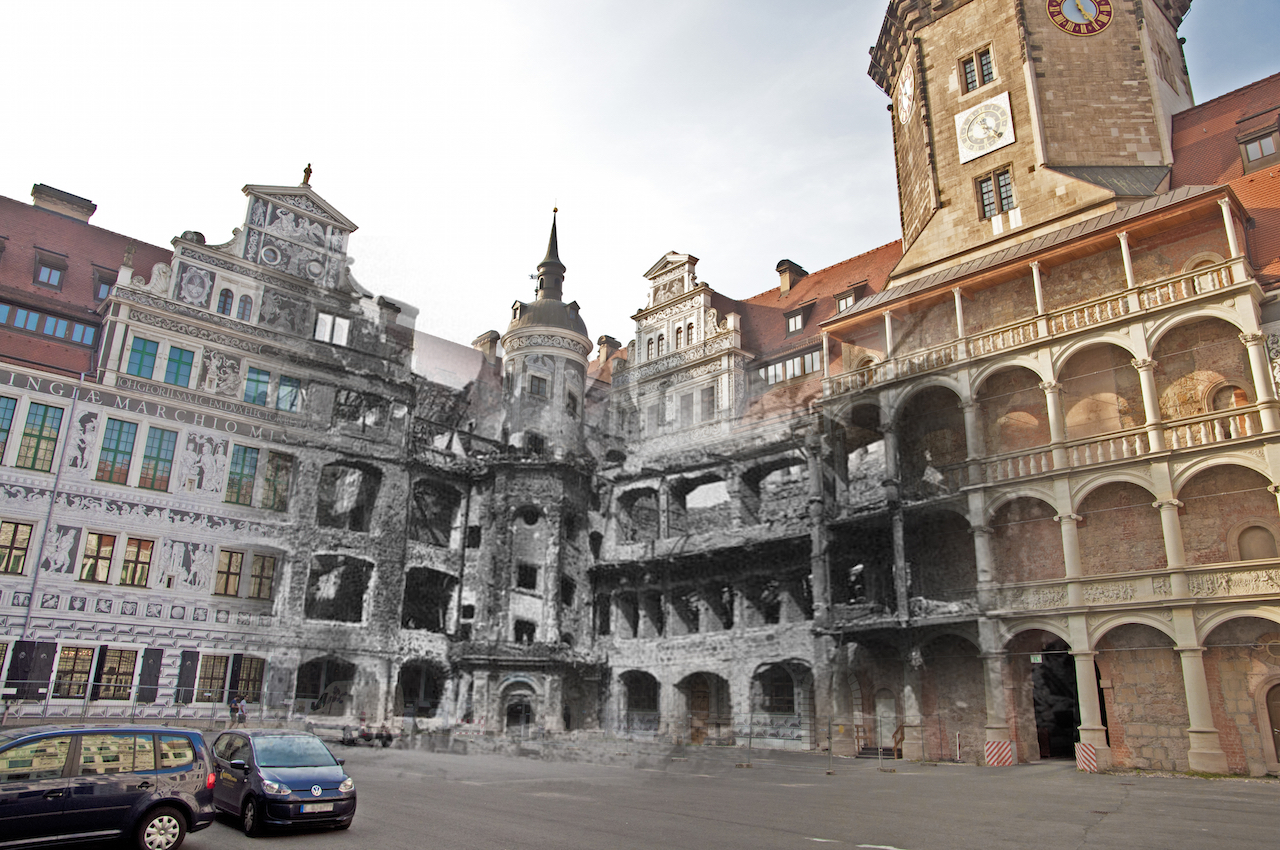
\includegraphics[width=\textwidth]{gfx/1945_2014_Residenzschloss_small.jpg}
   \caption{Residenzschloss Dresden, destroyed during World War II,
   \textcopyright\ Sergey Larenkov, printed with permission}
   \label{fig1}
\end{figure}

\begin{figure}
   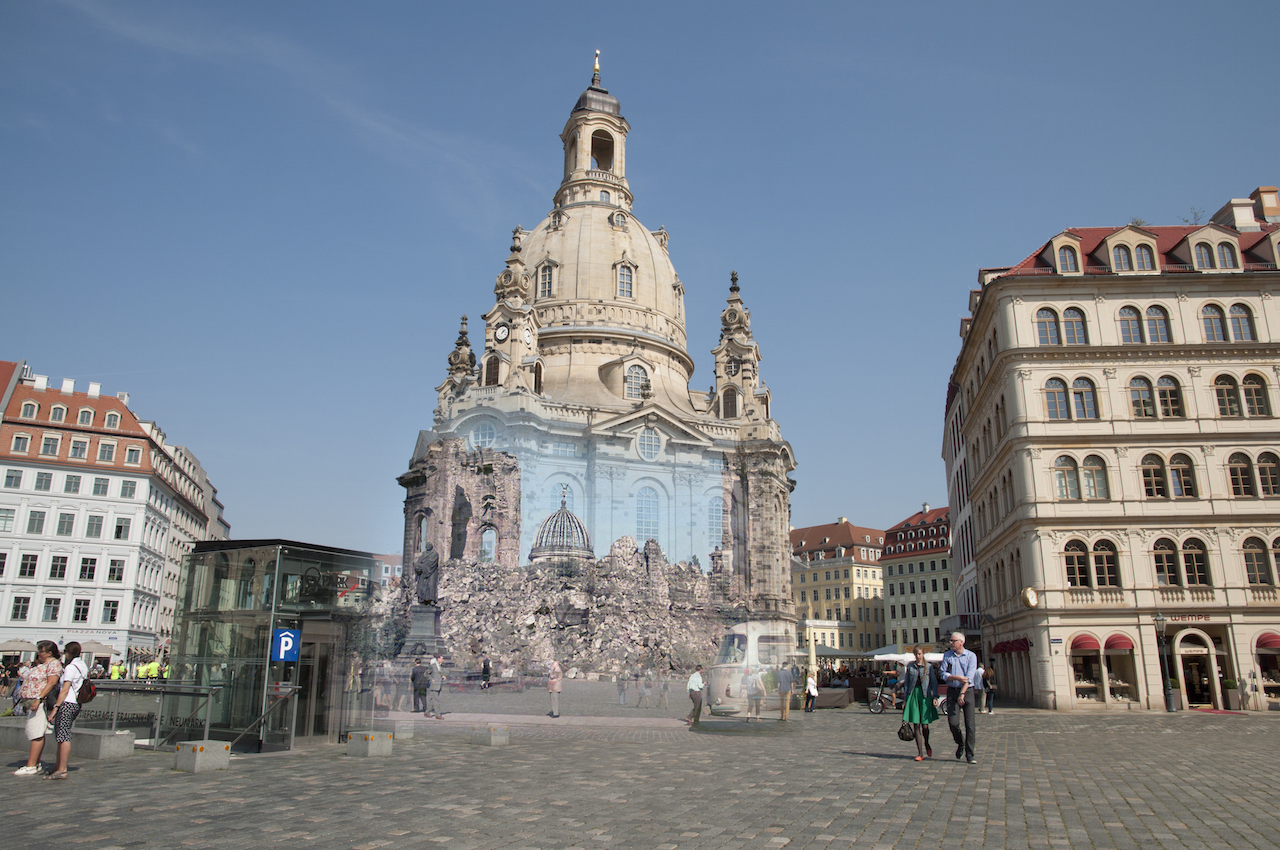
\includegraphics[width=\textwidth]{gfx/1950_2014_Frauenkirche_small.jpg}
   \caption{Frauenkirche Dresden, destroyed during World War II,
   \textcopyright\ Sergey Larenkov, printed with permission}
   \label{fig2}
\end{figure}

When done manually, the photographer must attempt to find the original viewpoint 
usually by visual inspection of the original image and trying to match the
current camera parameters---camera position, camera rotation, focal length,
possibly principal point---to the original.
The procedure is often carried out by placing the camera on a tripod and
comparing a printout of the original image with what can be seen through the
viewfinder or the camera screen. The number of parameters to match as well as
the difficulty to estimate them purely from comparing two-dimensional images makes the process
error-prone and tedious. Visual acuity and experience of the photographer thus
place limits on the accuracy with which the camera pose of the reference image
can be reconstructed. Some corrections can be done by post-processing the images
and warping the rephotograph with a homography to better match the original.

At the time of writing, few computerised aids are available to the photographer
(see below).  The advancement of mobile phones and tablet computers with
integrated cameras and larger screens presents the opportunity to develop
applications which can assist in this endeavour, moving away from the
traditional trial-and-error approach.  On current digital cameras
\footnote{At the time of writing, no commercial manufacturer produces a camera with
   user-modifiable firm- or software. A project at Stanford \citep{Levoy2010}
was discontinued \cite{FrankenCam}} 
this is impossible due to their closed
infrastructure not permitting running user programs. 

\section{Previous Approaches}

\subsection{Mobile Applications}

Two applications have been developed to assist a photographer in taking
rephotographs. For smartphone operating systems,
\emph{rePhoto}\footnote{\url{http://projectrephoto.com/}} and
\emph{Timera}\footnote{\url{http://www.timera.com/Explore}} exist, both
available for Android and iOS devices. These applications support the user by placing a transparent
version of the original image over the current camera image, allowing for easier
alignment. The captured rephotograph is then presented together with the
original image in a blend (c.f. \autoref{fig3}) which can be customized in
\emph{Timera}.

What is characteristical about both of these applications is that the user must still
determine on their own how to actually move the camera. An overlay simplifies
the procedure, eliminating some of the inaccuracy introduced into the manual approach by the
necessity to move the eyes from printout to camera, but it is still the user's
responsibility to determine the necessary motion between the current camera
position and the goal position (that of the original image). 

\subsection{Computational Re-Photography}

A more
sophisticated automated approach was presented in by MIT researchers in
2010. \citet{bae2010} found in preliminary studies that neither a side-by-side
view as would be used in the manual approach, nor a linear blend provided by
the above applications result in accurate rephotographs.

In this setup, the relevant parameters of a historic image's camera are
reconstructed, including the focal length, principal point and the six degrees
of freedom in camera pose. This subsection will give a high-level overview,
while a more in-depth discussion of the relevant concepts is deferred until
\autoref{chapter something}.

The software runs on a laptop connetcted to a digital camera.  After
reconstructing the scene in 3D by use of two images captured by the user, they
are then directed by the software to the desired viewpoint, the user does not
have to find it by themselves.  On the screen, they
are shown the current camera image alongside two arrows indicating in which
direction to move---one for movement in the sensor plane and one for movement
along the optical axis.

\citet*{bae2010} identify five primary obstacles in viewpoint reconstruction of a
historic photograph.
\begin{enumerate}
   \item The necessary camera motion has six degrees of freedom---three for
      translation and three for rotation---which are challenging for the user
      to adjust simultaneously, as changing one parameter will often necessitate
      adjustments for the others to improve the matching. Furthermore, the
      number of degrees of freedom makes it difficult to communicate to the
      user how they must move the camera.
   \item Computing relative translation between two cameras from corresponding
      image points is possible only up to an unknown scale (see
      \autoref{section on projective geometry}), meaning it is impossible to
      determine e.g. if an object viewed by the camera is small and close or
      large and further away. This poses the problem of how to determine if the
      user is close to the desired viewpoint and whether or not they have come
      closer or moved further away over iterations. 
   \item Relative pose estimation from corresponding points fails when the
      motion between the two cameras approaches zero, which is the ultimate goal
      one wishes to achieve. When na\"ivley comparing the current camera image
      to the reference photograph, the estimate for relative rotation and
      translation would become increasingly unreliable as the camera approaches the
      original viewpoint.
   \item Automated computation of relative camera pose will rely on feature
      detection to find correspondences. However, historical images will often
      be vastly different from the current scene. Not only may the scene itself
      have changed considerably, but also the historical image---having been
      taken by a historical camera---may differ in contrast, sharpness and
      colours. Feature detectors may not be able to reliably find
      correspondences when comparing an old with a new photograph.
   \item The calibration data---most importantly, focal length and principal
      point---of the historical camera are often unknown. The calibration data
      is needed for relative pose computation.
\end{enumerate}

Initially, after loading a historical image, the user is instructed to
take two photographs of the scene with a reasonably wide baseline (about
20\textdegree). One of them, termed \emph{first frame} is supposed to be
taken from some distance from the original viewpoint, the \emph{second
frame} should be the user's best eyeballed approximation of it. The wide
baseline allows for a more reliable 3D-reconstrution of the scene used to
tackle problems 2. and 3. 

SIFT features \citep{lowe2004} are computed and matched between the two images.
Given these correspondences, 3D coordinates of the points can be computed. A
selection of these is reprojected into the second frame after which the user
identifies six or more points in the historical photograph corresponding to
these points in the second frame. This allows estimating extrinsic and
intrinsic camera parameters of the historical camera by running an optimisation
algorithm on an initial estimate for relative rotation and translation between
first frame and reference image as well as sensor skew, focal length and
principal point of the historical camera (problem 5.).  The principal point's initial guess
is found again with help of the user who identifies three sets of parallel lines
in the historical image \citep[see][chapter 8.8]{h&z2004}.

The result is that the location of the reference camera relative to the first
camera is known. During the homing process, the current camera frame is compared
to the first frame (not the reference frame, avoiding problem 3.), which avoids
degeneracy due to the wide baseline. Given the locations of the reference camera
and the current frame's camera, each relative to the first frame, one can
compute the location of the reference relative to the current frame and thus
guide the user in the right direction. Hence, the reference photograph is not
needed anymore after this initial step, circumventing problem 4.

During homing, the current camera frame is warped according to the necessary
rotation before being shown to the user, allowing them to focus only on the
translation (problem 1.). This is possible since for rephotography
dealing with structures usually at some distance, the rotation will be small,
otherwise the warped image would be unusable.

A remaining problem (2.) is that the scale of the necessary translation is unknown,
so that only the direction is known. This poses the question of how to determine
whether the user has come closer to the goal or not. It may be feasible to find
the original viewpoint nonetheless, if it was possible to determine at least
when the user reaches it, but this impossible without further information. On
top of that, it would make for a better user experience if also the distance to
the goal could be communicated.

A key observation in this regard is that the actual scale of the translation is
irrelevant, it is sufficient that there be a way to make the scale consistent
accross iterations. That is, it is unnecessary to know whether the goal is a
specific distance aways, if one can ensure that the translations computed one
after the other can be somehow meaningfully compared. For this, Bae et. al
observe that when triangulating 3D coordinates from corresponding points, their
computed distance from the camera (the first frame) is inversely proportional
to the distance between the cameras. Therefore, in each iteration, the scale of
the world is computed by triangulating correspondences between the first and
current frames. The scale is compared to the scale computed in the initial step
for the first and second frames. Scaling the current translation vector by the
ratio of the two scales makes the length consistent across iterations and
decreasing with the distance to the goal.

The results of this method appear to be very successful, but two main drawbacks
exist.
\begin{itemize}
   \item The prototype is not very convenient, as it requires a (laptop)
      computer and a digital camera to carry out which is impractical for
      spontaneous rephotography.
   \item The application is not available to the public, neither in source nor
      binary form. It is therefore impossible to adapt it for more mobility.
\end{itemize}

\section{Goals of this thesis}

This work's objective can thus be summarised as follows.
\begin{enumerate}
   \item Implement in a prototypal fashion the process from \citep{bae2010} for
      a mobile operating system so it can be run on a smartphone or tablet and
      direct the user in approximate real-time.
   \item Evaluate the approach and attempt to reproduce the results.
\end{enumerate}

For a proof-of-concept application, several simplifying assumptions are made.
Firstly, it is assumed that the ``historic'' photograph is captured with the
same camera as the application is run on and that the camera is calibrated.
Secondly, no strong visual differences between the reference and current scenes
are assumed so that the reference image is accessible to the same feature
detection algorithm without the user manually labelling correspondences. 

The application targets iOS 8 and current hardware, as image processing is
computationally intense, and has been tested on an iPad Air 2.


\chapter{Camera Geometry}

This chapter will introduce the geometry of image projection, largely following
\citep[chapters 6,7]{h&z2004} and the geometry of two views (the epipolar
geometry, \citet[chapter 5.1]{ma2003}) and
how it can be used to recover relative camera position from two images of the
same scene. It largely follows.

\section{Camera Models}

The camera model used is the ideal pinhole camera model which postulates several
idealised assumptions.
\begin{enumerate}
   \item The aperture size is infinitely small
   \item There are no lens effects (\emph{thin lens} assumption)
   \item The angle of view is arbitrarily large
   \item All world points projected onto the image plane are in focus, owing to
      the small aperture
\end{enumerate}

\marginnote{Homogeneous vectors are
the elements of projective geometry. They can be obtained from cartesian
coordinates by appending a 1-element. All projective entities which differ only
by a scalar factor are equivalent, one writes $\mbf{x} \sim \mbf{y}$ if
$\mbf{x} = \lambda\mbf{y}, \lambda \neq 0$. This has the added effect that
points at infinity can be represented by vectors whose last coordinate is zero.}

Given a camera $C$ whose center of projection is the origin and a point
$\mbf{X}$ in camera-centric coordinates, the central projection of
$\mbf{X}$ onto $C$'s image plane is depicted in a side-view in
\autoref{pinhole}.  The image plane is virtually moved to the front of the
camera, otherwise the image would be mirrored at the principal point as in real
cameras.  Let $f$ be the focal length, which is the distance of the image plane
to the optical centre.  If $\mbf{X} = (X,Y,Z)$, then $x=\left(f \frac{X}{Z},
f \frac{Y}{Z}, f\right)$ by use of the intercept theorem.%, with $\left(fX, fY\right)^T$ being the coordinates in the image plane.


\begin{figure}[h]
   {\centering      
      \begin{tikzpicture}[every node/.style={outer sep=0,inner sep=0},
   label distance=5pt]
   \usetikzlibrary{calc}
   \fill (0,0) circle (2pt) node[label=below:{$C$}] (C) {};
   \draw[->,name path=y-axis] (C) -- ++(0,4cm);
   \draw[->,name path=x-axis] (C) -- ++(8cm,0);

   \fill (7cm,3cm) circle (2pt) node[label=above right:{$\mathbf{X}$}] (X) {};

   \draw[name path=image plane] (3cm,1.7cm) -- ++(0,-2*1.7cm);

   \draw[|-|] (0,-2cm) -- (3cm,-2cm) node[midway,below=1em] (f) {$f$};

   \draw[name path=ray] (C) -- (X);
   \fill[name intersections={of=ray and image plane}]
   (intersection-1) circle (2pt) coordinate (c);
   \node[label=above left:{$x$}] (x) at (c) {};

   \draw[dashed] (0,3cm) node[left=1em] {$Y$} -- (X) -- (7cm,0)
   node[below=1em]
   {$Z$};

   % \draw[|-|] (0,-3cm) -- (7cm,-3cm) node[midway,below=1em] (Z) {$Z$};

   \draw[|-|,name intersections={of=x-axis and image plane}] (x) ++(1em,0) --
   ($(intersection-1) + (1em,0)$) node [right=1em,midway] {$f \cdot
   \frac{Y}{Z}$};

\end{tikzpicture}

      \caption{Central projection for a pinhole camera}
   \label{pinhole}}
\end{figure}


When representing the points as homogeneous quantities, the central projection
can be expressed by a matrix multiplication. 
This can be written with homogeneous coordinates as
\begin{IEEEeqnarray}{rCl} \label{eq:projection}
      \left(
         \begin{array}{c}
            fX \\ fY \\ Z
         \end{array}
      \right) & = & \underbrace{\addstackgap[6pt]{\left(
         \begin{array}{cccc}
            f & 0 & 0 & 0 \\
            0 & f & 0 & 0 \\
            0 & 0 & 1 & 0
         \end{array}
\right)}}_{\text{Projection Matrix of $C$}} \left(\begin{array}{c} X \\ Y \\ Z \\ 1 \end{array}\right)
\end{IEEEeqnarray}

or in short
\begin{equation}
   \mbf{x} \sim P\mbf{X}
\end{equation}

% If the unit of the coordinatesystem is chosen to be $f$, then the image plane is
% $Z = f$ and 
% \eqref{eq:projection} becomes
% \begin{IEEEeqnarray}{rCl}
%       \left(
%          \begin{array}{c}
%             X \\ Y \\ \frac{z}{f}
%          \end{array}
%       \right) & = & \addstackgap[6pt]{\left(
%          \begin{array}{cccc}
%             1 & 0 & 0 & 0 \\
%             0 & 1 & 0 & 0 \\
%             0 & 0 & \frac{1}{f} & 0
%          \end{array}
% \right)} \left(\begin{array}{c} X \\ Y \\ Z \\ 1 \end{array}\right)
% \end{IEEEeqnarray}

\subsection{Camera Extrinsics}

The above situation is a special case wherein the camera centre $C$ defines the
origin and the optical and image axes are the coordinate axes. Thus, the rotation
and translation of the camera relative to this coordinate system is zero. More
generally, there might be a world coordinate frame with different origin 
and different axes, so that a coordinate transform must be applied to $\mbf{X}$
before the projection. 

Let $R \in \mathbb{R}^{3\times3}$ be a rotation matrix
giving the camera's rotation relative to the world frame and $t \in
\mathbb{R}^{3\times1}$ its translation such that

\begin{equation}
   \mbf{X}_{\text{cam}} = R \mbf{X}_{\text{world}} + t
\end{equation}

Then the projection of a point $\mbf{X}$
in world coordinates onto the image plane becomes

\begin{IEEEeqnarray}{rCl}
   \mbf{x} & = & P \mbf{X}\\
   \mbf{x} & = & \left(\begin{array}{ccc}
   f & 0 & 0 \\
   0 & f & 0 \\
   0 & 0 & 1
   \end{array}\right) \left[R \mid t\right] \mbf{X} \label{eq:projection_rt}
\end{IEEEeqnarray}

\subsection{Camera Intrinsics}
\label{subsec:intrinsics}

Above, the resulting image points $\mbf{x}$ were in \emph{normalised} image
coordinates. In particular, the
principal point---the
intersection of the image plane with the optical axis---was assumed to be
$(0,0)$. But generally, image coordinates are expressed in pixels relative to
the upper left corner of the sensor. To convert between normalised and pixel
coordinates, 
the camera's five intrinsic parameters and can be written in matrix form and
premultiplied in \eqref{eq:projection_rt} as
\begin{IEEEeqnarray}{rCl}
   \mbf{x} & = & \left(
   \begin{array}{ccc}
      s_x & s     & c_x \\
      0   & s_y   & c_y \\
      0   &       & 1
   \end{array} 
\right) \left(\begin{array}{ccc}
   f & 0 & 0 \\
   0 & f & 0 \\
   0 & 0 & 1
\end{array}\right) \left[R \mid t\right] \mbf{X}
\end{IEEEeqnarray}
where $s_x$ and $s_y$ are the focal lengths in $x$- and $y$-directions expressed
in pixel units per world unit (e.g. cm; $s_x$ and $s_y$ are not necessarily identical, if the sensor has
non-square pixels), $s$ the sensor skew (the pixels may not be rectangular;
their edges may not be perpendicular) which is usually zero, and the coordinates
of the principal point $(c_x,c_y)$ with respect to the origin of the image plane
which usually placed at the upper left corner.
The intrinsic camera parameters are assembled in
\begin{IEEEeqnarray}{rCl}
   K & = & \left(\begin{array}{ccc}
   fs_x & s & c_x \\
   0 & fs_y & c_y \\
   0 & 0 & 1
\end{array}\right)  
\end{IEEEeqnarray}
are therefore essential to
relate world points to image points which will be important for this
application. The normalised coordinates $\hat{\mbf{x}}$ for a pixel coordinate
$\mbf{x}$ can be computed as
\begin{equation}
   \hat{\mbf{x}} = K^{-1}\mbf{x},
\end{equation}
which will remove the effects of the calibration parameters and thus make the
image coordinates independent of the camera's internal characteristics.

In theory, these parameters could be obtained from the camera's
vendor who knows the precise manufacturing specifications. In practice, only the
focal lengths $f_x, f_y$ are known, in most cases only one with the assumption
of square pixels. Usually, the principal
point is assumed to be at the sensor centre and the pixels are assumed to be
rectangular. In practice however, there are variances introduced by different
causes such as imprecise manufacturing or physical impacts which may decentre
the lens such that the principal point is no longer at the centre. 

A further compilcation is introduced by the camera lens which will often have a
non-negligible distortion, most prominently radial distorion as depicted in
\autoref{distortion}. It can be modeled by the application of a 
distortion factor to the ideal undistorted image coordinates $(\tilde{x}, \tilde{y})$.

\begin{figure}
   {\centering      
      \begin{tikzpicture}[every to/.style={color=red}]

   \makegrayinprint

   \newcommand{\yshift}{6cm}
   \draw (0,0) rectangle (4,3);
   \begin{scope}[xshift=2cm,yshift=1.5cm]
      \draw (-1.5,-1) to[bend right=8] (1.5,-1) to[bend right=8] (1.5,1) to[bend
      right=8] (-1.5,1) to[bend right=8] (-1.5,-1);
   \end{scope}
   \begin{scope}[xshift=\yshift]
      \draw (0,0) rectangle (4,3);
      \begin{scope}[xshift=2cm,yshift=1.5cm]
         \draw (-1.5,-1) to (1.5,-1) to (1.5,1) to (-1.5,1) to (-1.5,-1);
      \end{scope}
   \end{scope}
\draw[-{Latex},thick,color=RoyalBlue,text=black] (4,1.5) ++(1mm,0) -- node[below,midway,font=\footnotesize]
   {correction} ($(\yshift,1.5) - (1mm,0)$);
\end{tikzpicture}

   \caption{Radially distorted image on the left, the corrected image on the
   right.}
   \label{distortion}}
\end{figure}


\begin{equation}
   \begin{pmatrix}
      x_d \\ y_d
   \end{pmatrix} = L(r)\begin{pmatrix}
      \tilde{x} \\ \tilde{y}
   \end{pmatrix}
\end{equation}

where $L$ is a nonlinear function of the distance $r$ from the distortion
center---usually coincident with the principal point. The function can be
approximated as an exponential with a Taylor expansion
\begin{equation}
   L(r) = 1 + \sum\limits_{i=1}^k \kappa_i r^i
\end{equation}
for a given $k$ \citep[see][chapter 7.4]{h&z2004}. The intrinsic camera
parameters which consist in the entries of $K$ and distortion coefficients
$\kappa_i$ must be determined in order to accurately relate world coordinates to
image coordinates. They can be found by calibrating the camera. Different
methods exist \citep[e.g][]{zhang2000} but will not be examined here.

\section{Epipolar Geometry}

Epipolar geometry is the geometry which relates the image points in two views of
the same scene. \autoref{epipolar} shows the basic setup. 

We consider a scene viewed by two cameras with optical centres $c_1$ and $c_2$,
where $c_1$ defines the origin,
world points $\mbf{X}_i\in\mathbb{R}^3$, where the subscript denotes the coordinate
frame---the first camera, arbitrarily chosen to be the left one, or the second
camera---and homogeneous image points $\mbf{x}_i$ which are the projections of $\mbf{X}_i$
onto the image planes and thus correspond to the same world point. The cameras
are related by a rigid body transform $(R,T)$, where $R$ is a $3\times3$
rotation matrix and $T$ the translation between the camera centres. Throughout
this work, the direction of coordinate frame transformation will be such that
\begin{equation}\label{eq:camera_transform}
   \mbf{X}_2 = R\mbf{X}_1 + T.
\end{equation}

It is obvious that the following relation holds,
\begin{equation}\label{eq:project_world_point}
   \lambda_i\mbf{x}_i = \mbf{X}_i, ~\lambda_i > 0
\end{equation}
that is, the world point lies on a ray through the optical centre and the image
point. 

\begin{figure}[h]
   {\centering      
      \usetikzlibrary{intersections, calc, arrows.meta}
\begin{tikzpicture}[every node/.style={outer sep=0,inner sep=0},
   label distance=5pt]
   \def\baseline{10cm}
   \draw[fill] (0,0) circle (2pt) node[label=below left:{$c_1$}] (c1) {};
   \draw[fill] (\baseline,0) circle (2pt) node[label=below left:{$c_2$}] (c2) {};

   \newcommand{\sensorplane}[1]{
      \path[name path=#1,draw] (1cm,0.5cm) -- (1cm,2.5cm) -- (3.5cm,1cm) -- (3.5cm,-1cm) -- cycle
   }
   \begin{scope}
      \sensorplane{plane1};
   \end{scope}

   \begin{scope}[yscale=1,xscale=-1,xshift=-\baseline]
      \sensorplane{plane2};
   \end{scope}

   \fill (0.5*\baseline,3cm) circle (2pt) node[label=above:{$\mathbf{X}_1$}]
   (X1) {};

   \draw (c1) -- ++(3cm,0) [fill] circle (2pt) node[label=above:{$e_1$}] (e1)
   {} coordinate (c);
   \draw[dotted] (c) -- (3.5cm,0) coordinate (c);
   \draw[solid] (c) -- (\baseline-3.5cm,0) coordinate (c);
   \draw[dotted] (c) -- (\baseline-3cm,0) coordinate (c);
   \draw[fill] (c) circle (2pt) node[label=above:{$e_2$}] (e2) {} -- (c2);

   % lines from camera center to x
   \path[name path=c1 to X1] (c1) -- (X1) coordinate[pos=.3] (c);
   \draw[solid,fill] (c1) -- (c) coordinate (x1) circle (2pt);
   \node[label=above:{$x_1$}] (x1) at (c) {};
   \draw[dotted,name intersections={of=c1 to X1 and plane1}] (c) --
   (intersection-2) coordinate (c);
   \draw[solid] (c) -- (X1);

   \path[name path=c2 to X1] (c2) -- (X1) coordinate[pos=.3] (c);
   \draw[solid,fill] (c2) -- (c) coordinate (x2) circle (2pt);
   \node[label=above:{$x_2$}] (x2) at (c) {};
   \draw[dotted,name intersections={of=c2 to X1 and plane2}] (c) --
   (intersection-2) coordinate (c);
   \draw[solid] (c) -- (X1);

   % draw epilines
   \draw[RoyalBlue,text=black] (e2) -- (x2) node[midway,label=above:{$l_2$}] (label-l2) {};

   \draw[RoyalBlue,text=black] (e1) -- (x1) node[midway,label=above:{$l_1$}] (label-l1) {};

   % draw relative rotation and translation
   \draw[-{Latex}] ($(c1) + (2em,-2em)$) to[bend right=50] node[below=1em, midway]
   {$R$, $T$} ($(c2) + (-2em,-2em)$);

\end{tikzpicture}

      \caption{Basic epipolar geometry with camera centres $c_1$, $c_2$, image
      points $\mbf{x}_1$, $\mbf{x}_2$, a world point $\mbf{X}_1$, epipoles
   $e_1$, $e_2$ and epipolar lines $l_1$, $l_2$}
   \label{epipolar}}
\end{figure}

Given the corresponding points $\mbf{x}_i$ in two images, the ultimate goal is
to retrieve the euclidean transform $(R,T)$.

In case the image coordinates for both cameras are normalised (c.f.
\autoref{subsec:intrinsics}), they have equal units, so
starting from \eqref{eq:camera_transform}, one can derive
\begin{IEEEeqnarray*}{rClls}
   \mbf{X}_2 & = & R\mbf{X}_1 + T & \hspace {2cm} \\
   \lambda_2\mbf{x}_2 & = & R\lambda_1\mbf{x}_1 + T & & (by \eqref{eq:project_world_point}) \\
   \lambda_2\widehat{T}\mbf{x}_2 & = & \widehat{T}R\lambda_1\mbf{x}_1 + \widehat{T}T & &
   $\widehat{T}\in\mathbb{R}^{3\times3}$ with $\widehat{T}\mbf{x} = T \times
   \mbf{x}$ \\
   \lambda_2\mbf{x}_2^T\widehat{T}\mbf{x}_2 & = &
   \mbf{x}_2^T\widehat{T}R\lambda_1\mbf{x}_1 + 0 & & $T \times T = 0$ \\
   \lambda_2\cdot 0 & = &
   \mbf{x}_2^T\widehat{T}R\lambda_1\mbf{x}_1 & & $\widehat{T}\mbf{x}_2$ is
   perpendicular to $\mbf{x}_2$ \\
   0 & = & \mbf{x}_2^T\underbrace{\widehat{T}R}_{E}\mbf{x}_1
   \label{eq:epiconstraint}\IEEEyesnumber
\end{IEEEeqnarray*}

The product $E=\widehat{T}R$ is the essential matrix and the constraint it
imposes on corresponding image points the essential constraint
\citep[see][chapter 5]{ma2003}. 

An intuition for the essential matrix can be
obtained from \autoref{epipolar}. Given an image point in one frame $\mbf{x}_1$,
in attempting to find the point $\mbf{x}_2$ corresponding to the same world
point $\mbf{X}_1$, the epipolar geometry restricts the search space to one
dimension---the epipolar line of $\mbf{x}_1$ in the second camera's image plane.
The camera centres and the world point define an epipolar plane. The
backprojection of $\mbf{x}_1$ is the ray through $\mbf{x}_1$ and the optical
centre $c_1$. All points on this ray are mapped to the same point on the image
plane of $c_2$. Depending on how far away the world point $\mbf{X}_1$ is from $c_1$, its
image on the second camera's image plane will vary---but it will be on the
intersection of the image plane and the epipolar plane, the epipolar line of
$\mbf{x}_1$. The line $l_1$ may be identified with its coimage (the orthogonal
complement of its preimage) $l_1 = e_1 \times \mbf{x}_2 \in \mathbb{R}^3$ so that

\begin{equation} \label{eq:epiline}
   \forall\mbf{x}: \mbf{x}\in l_1 \Leftrightarrow \mbf{x}^T\cdot l_1 = 0.
\end{equation} 

The coimage of the epipolar line is the vector perpendicular to the epipolar plane,
so every vector in this plane will have an inner product of $0$ with this
vector. Constrained to vectors in the image planes, this means that all vectors on the
epipolar line will have an inner product of $0$ with this vector $l_1$.
Referring back to \eqref{eq:epiconstraint}, it can be seen that multiplication
with $E$ will yield a term $\mbf{x}_2^TE = l$ which fulfills 
\begin{equation}
   l \cdot \mbf{x}_1 = 0,
\end{equation}
which is precisely the relation stated in \eqref{eq:epiline}. The essential
matrix thus maps an image point onto its epipolar line in the other image.

\section{Essential Matrix Estimation}

Estimating the essential matrix between two
cameras and decomposing it into relative rotation and translation is a necessity
in the endeavour to communicate a necessary camera movement to the application's
user. The most prominent algorithms in this regard are the 8-Point algorithm
introduced in its original form by \citet{longuet-higgins1987} and improved upon
by \citet{hartley1997}, and the 5-Point algorithm proposed by
\citet{nister2004}. To illustrate the mathematical tractability of the problem,
the former will be presented below.

\subsection{The 8-Point Algorithm}

The essential matrix has nine elements, but since all image coordinates are
projective quantities, the set of all essential matrices differing by a constant
factor is equivalent so that one degree of freedom is removed and at most eight
remain. If one were to formulate constraints on the elements as a system of
linear equations, eight of those should be sufficient to uniquely determine an
essential matrix. An improvement suggested in \citep{hartley1997} is the
precpocessing of the input data (the image coordinates) by translation and
scaling. This improves the robustness of the algorithm, but will be omitted
here.

For each point correspondence $\{\mbf{x}_1 = (x_1,y_1,1),\mbf{x}_2 = (x_2, y_2,
1)\}$, one linear equation
\begin{equation}
   \mbf{x}_2^T E \mbf{x}_1 = 0
\end{equation}
is generated, which can be rewritten as
\begin{IEEEeqnarray*}{rCcCcCc}
   0 & = & x_2 x_1 e_{11} & + & x_2 y_1 e_{12}  & + &  x_2 e_{13} \\
     & + & y_2 x_1 e_{21} & + & y_2 y_1 e_{22} & + & y_2 e_{23} \\
     & + & x_1 e_{31} & + & y_1 e_{32} & + & e_{33} \label{eq:linear_equation}
   \IEEEyesnumber
\end{IEEEeqnarray*}
Let $\mbf{e}$ denote the vector of $E$'s entries in row-major order, then
\begin{equation}
   0 = \left( x_2 x_1, x_2 y_1, x_2, y_2 x_1, y_2 y_1, y_2, x_1, y_1,
   1\right)\cdot\mbf{e}
\end{equation}

If $n$ correspondences are given, they each contribute one row to
\begin{IEEEeqnarray}{rCl}
   A\mbf{e} & = & \left[ \begin{array}{ccccccccc}
      x_2^1 x_1^1 & x_2^1 y_1^1 & x_2^1 & y_2^1 x_1^1 & y_2^1 y_1^1 & y_2^1 & x_1^1 & y_1^1 & 1 \\
   \vdots & & & & & & & & \vdots \\
      x_2^n x_1^n & x_2^n y_1^n & x_2^n & y_2^n x_1^n & y_2^n y_1^n & y_2^n & x_1^n & y_1^n & 1
\end{array} \right] \mbf{e} = 0 \nonumber\\*\label{eq:stacked_essential}
\end{IEEEeqnarray}

For eight noise-free point correspondences in general position, there is a
unique solution, but in practice, one uses more correspondences and the system
is overdetermined, so a least-squares-solution minimising $\vert\vert A\mbf{e}
\vert\vert = \sum_{ij} (A\mbf{e})_{ij}^2$ is sought. 
The solution is unique up to scale, since all multiples of $\mbf{e}$ will
satisfy \eqref{eq:stacked_essential}. One therfore introduces the constraint
$\vert\vert \mbf{e} \vert\vert = 1$ which also excludes a trivial zero solution.

This solution vector is the singular
vector with the smallest singular value in the singular value decomposition of
$A$ or equivalently, the smallest eigenvector of $A^TA$ \citep[see]{hartley1997}
and thus can be found by Singular Value Decomposition.

\subsection{Further Algorihtms}

The 8-Point Algorithm is mathematically straightforward and linear, but in
practice it suffers from noise \citep[e.g.][see]{chen2000} and in real
applications approaches the robustness of other methods only in its normalised
form from \citep{hartley1997}. As such, many other methods exist. A review of
many methods is given in \citep{zhang1998}.


chapter{Challenges In Relative Pose Estimation}

The success of recovery of relative pose mainly depends on two factors: The
accuracy and correctness of image point correspondences and them not being in
a degenerate configuration, so that they provide enough information about the
scene.

This chapter will examine the preconditions and the feasibility of pose recovery
in realistic conditions. Several problematic cases will be identified and
described. Furthermore, an assessment of different feature detection algorithms
for the purpose of this work will be given.

\section{Degenerate Configurations}

Degenerate configurations are those in which the data on which the essential
matrix is estimated allows for more than one mathematically valid solution. Two
different cases can be observed.

\subsection{Structure degeneracy}

Structure degeneracy is a configuration of points in the observed scene which do
not provide enough information to wholly determine an essential matrix. The
projection matrix $P\in\mathbb{R}^{3\times3}$ with 
\begin{equation*}
   \mbf{x} = P\mbf{X}
\end{equation*}
has twelve elements but is a projective quantity, so all non-zero multiples of
$P$ are equivalent, wherefore it has only eleven degrees of freedom.  A
degenerate case is for instance when all points observed by the two cameras lie
on the same plane (or worse, a subspace of even lower dimension). The images of
a planar surface in two cameras as well as the planar surface itself and its
image are related by a homography \citep[see][ch. 13]{h&z2004}, which is a
mapping between planes and has eight degrees of freedom (being a $3\times3$
matrix and a projective element), meaning that three degrees of freedom are
undetermined \citep{torr1999}.  A set of coplanar points thus does not provide
enough information to uniquely determine an epipolar geometry. 

There are approaches to deal with this problem (e.g. an algorithm developed by
\citet{chum2005} or \citet{decker2008}), but the standard approaches such as
the five point solver with RANSAC implemented in OpenCV are susceptible to this
situation.

\subsection{Motion Degeneracy}

A second type of degeneracy occurs when the camera motion between two images has
fewer degrees of freedom than the model to be estimated---the essential matrix.
If the camera only translates or only rotates between images, the motion has
maximally three degrees of freedom. As \citet{decker2008} point out, an
essential matrix estimated under such conditions could be consistent with all
correct point matches, but also with some false ones due to the mismatch in
degrees of freedom between data and model. In schemes like RANSAC, such an
estimate will have a large consensus set---all inliers \emph{plus}
outliers---and so may lead to the termination of the algorithm, despite being
inaccurate.

It is unlikely in rephotography that the observed scene will be completely
planar, or that the user will move from the first frame in a motion which is
pure rotation or translation, these degeneracies can be labelled edge cases and
are not specifically handled in the application.

\section{Finding Correspondences}

There is a variety of automatic feature detection algorithms which differ in
repeatability, robustness to noise, speed and invariance with respect to image
characteristics such as scale, brightness, or rotation. 
Generally, a feature detector identifies potentially salient points in an image
and computes a descriptor for these points in a way that the same point under
different conditions will yield an ideally identical descriptor. When points of
interest---usually called \emph{keypoints}---are available in multiple images,
their descriptors can be compared and the best match according to some metric
can be selected for each keypoint. The matches found can then be used as
corresponding points for relative pose estimation.

Classical state-of-the-art detectors include e.g. SIFT \citep{lowe1999}, SURF
\citep{bay2006} which both compute real-valued descriptors. A natural criterion
for selecting the best matching keypoint for a given keypoint is the $L_2$-norm
of the difference of their descriptors, which is a relatively expensive
operation. While e.g. SURF improves performance over the computationally
demanding SIFT detector, the speed of matching can still present a bottleneck in
time-critical contexts.

\subsection{SIFT}

\subsection{AKAZE}




\chapter{Evaluation}

The approach has been evaluated on two realistic datasets. The most important
questions are whether the direction of the necessary translation is correctly
identified and its scale decreasing with distance to the target.
For both sets of images, the ground-truth translation between each image and the
first frame has been measured with centimetre accuracy, while the ground-truth
rotation has been estimated from manually labeled correspondence as it is
difficult to measure without the proper instruments. Since for the case of
noise-free correspondences in a non-degenerate configuration, relative pose
estimation algorithms are mathematically correct, this has been deemed
sufficiently accurate to evaluate the procedure. For each image pair, 19--27
correspondences have been labeled, of which the majority is used for pose
recovery. For pose recovery, RANSAC is used in conjunction with the five-point
solver, a point is considered an inlier for a given essential matrix if its
distance to its epipolar line is no more than three pixels. These parameters
lead to the majority of points being inliers of the pose recovery, the few
outliers can be explained by imprecise labeling.

In both data sets, the translation was mostly in the horizontal direction and
along the optical axis; the vertical translation is thus neglected. Similarly,
rotation was applied mainly around the vertical axis.

In order to idealise the condition, the reference photograph has been used to
fill the role of the second frame for world scale computation. In reality, since
the reference location is unknown, the reference world scale is obtained from a
position somewhat off.

\section{Train Station Data Set}

A schematic bird's eye view of the captures is shown in \autoref{fig:train_data_scenario}.

\begin{figure}
   {\centering      
      \begin{tikzpicture}
   \begin{axis}[
         xmin = -1,
         xmax = 6,
         ymin = -1,
         ymax = 6,
         xlabel = $x$,
         ylabel = $y$,
         every node near coord/.append style={yshift=-0.5cm,anchor=-10} % hacky way putting nodes below points instead of above
      ]
      \addplot+[
         nodes near coords,
         only marks,
         point meta=explicit symbolic,
      ]
      coordinates {
         (0,0)        [0]
         (5.65,2.65)  [1]
         (3.12,0.16)  [2]
         (0.83,0.03)  [3]
         (0.20,0.03)  [4]
         (2,5)        [station]
      };

      \coordinate (station) at (axis cs:2,5);

      \foreach \x / \y in {0/0,5.65/2.65,3.12/0.16,0.83/0.03,0.20/0.03}
      {
         \edef\temp{
            \noexpand\node[outer sep=0,inner sep=0] (foo) at (axis cs:\x,\y) {}; 
         \noexpand\draw[->] (foo) -- ($ (foo) !1cm! (station) $);
      }
         \temp
      }

   \end{axis}
\end{tikzpicture}

      \caption{Schematic representation of the train data set. Lengths and angles are not
      precise.}
   \label{fig:train_data_scenario}}
\end{figure}
\autoref{tab:train_data} summarises the ground truth for the five images.

\subsection{Scale Estimation}

\autoref{fig:train_KAZE_dist_ratio} shows how the average distance of points to the first
frame's camera varies with the second image used for triangulation. The plot
illustrates that---especially at full resolution---the ratio based on feature
matching closely mirrors the real value. The difference increases with
decreasing image scale, but the the slope of the graphs is quite similar. This
shows that indeed with increasing distance to the first frame, the ratio
decreases, allowing a deduction as to how close the camera is to the target, at
least with respect to previous iterations. The situation is somewhat worse at
the smallest scale with the ratio between the fifth third and fourth images
barely decreasing.

\newcolumntype{m}{>{$}c<{$}}

\begin{table}
   \caption{Ground truth for the train data. Image 0 is the reference frame,
   translations and rotations are given as in \eqref{eq:camera_transform}.}
   \begin{tabular}{cmmm}
      \toprule
      Image        & \text{Translation to reference} & \text{Rotation to reference} & \text{ratio}\\
      number       & [x,y,z]                         & [\theta_x, \theta_y, \theta_z]
      \\
      \midrule
      0 & [0      , 0 , 0]      & [0        , 0       , 0]       & 1\\
      1 & [ .9053 , 0 , .4246 ] & [ -3.3779 , -9.3779 , 1.05121] & 3.8936\\
      2 & [ .9986 , 0 , .0512 ] & [ -1.3274 , -5.7134 , -.1884 ] & 1.6461\\
      3 & [ .9993 , 0 , .0361 ] & [ -1.7156 , -2.4761 , .3469  ] & 1.0965\\
      4 & [ .9950 , 0 , .0995 ] & [ .054606 , -4.4867 , .2452  ] & 1.0343\\
   \end{tabular}
   \label{tab:train_data}
\end{table}

\begin{figure}
   {\centering      
      \pgfplotstableread[col sep=space]{data/bahnhof_detector_KAZE_resize_1_ratio_0.800000.dat}\datatablenoresize
\pgfplotstableread[col sep=space]{data/bahnhof_detector_KAZE_resize_2_ratio_0.800000.dat}\datatableresize
\pgfplotstableread[col sep=space]{data/bahnhof_detector_KAZE_resize_4_ratio_0.800000.dat}\datatabledoubleresize
\begin{tikzpicture}
   \begin{axis}[
         xlabel={Image Number},
         ylabel={Distance ratio},
         ymax=4.5,
         xtick=data,
         % xticklabels from table={\datatable}{fname}
         scale=.6, % dare you to change this to sth larger
         legend pos=north east,
      ]

      % original size
      \addplot table[
         x expr=\coordindex,
         y=realdist_ratio,
      ] {\datatablenoresize};
      \addlegendentry{Truth}

      \addplot table[
         x expr=\coordindex,
         y=dist_ratio,
      ] {\datatablenoresize};
      \addlegendentry{$s=1$}

      % scaled by 2
      \addplot table[
         x expr=\coordindex,
         y=dist_ratio,
      ] {\datatableresize};
      \addlegendentry{$s=2$}

      % scaled by 2
      \addplot table[
         x expr=\coordindex,
         y=dist_ratio,
      ] {\datatabledoubleresize};
      \addlegendentry{$s=4$}

   \end{axis}
\end{tikzpicture}

      \caption{Evolution of the distance ratio between images in the Train Station
      data set with KAZE features}
   \label{fig:train_KAZE_dist_ratio}}
\end{figure}

\section{Manor Data Set}

The schematic positions for the seven manor captures (including reference
photograph) are shown in \autoref{fig:manor_data_scenario}. In contrast to the
train station, there is prominent movement along the optical axis.

\begin{figure}
   {\centering      
      \begin{tikzpicture}
   \begin{axis}[
         xmin = -2,
         xmax = 20,
         ymin = -10,
         ymax = 16,
         xlabel = $x$,
         ylabel = $y$,
         every node near coord/.append style={anchor=5} % hacky way putting nodes below points instead of above
      ]
      \addplot+[
         nodes near coords,
         only marks,
         point meta=explicit symbolic,
         mark=*,
         black,
      ]
      coordinates {
         (0,0)   [0]
         (2,0)   [1]
         (4,2)   [2]
         (4,4)   [3]
         (8,-5)  [4]
         (10,4)  [5]
         (16,-6) [6]
         (16,2)  [first frame]
         (10,15) [manor]
      };

      \coordinate (manor) at (axis cs:10,15);

      \foreach \x / \y in {0/0,2/0,4/2,4/4,8/-5,10/4,16/-6,16/2}
      {
         \edef\temp{
            \noexpand\node[outer sep=0,inner sep=0] (foo) at (axis cs:\x,\y) {}; 
            \noexpand\draw[->] (foo) -- ($ (foo) !.5cm! (manor) $);
         }
         \temp
      }

   \end{axis}
\end{tikzpicture}

      \caption{Schematic representation of the manor data set. Lengths and angles are not
      precise.}
   \label{fig:manor_data_scenario}}
\end{figure}

\begin{table}
   \caption{Ground truth for the manor data. Image 0 is the reference frame,
   translations and rotations are given as in \eqref{eq:camera_transform}.}
   \begin{tabular}{cmmm}
      \toprule
      Image        & \text{Translation to reference} & \text{Rotation to reference} & \text{ratio}\\
      number       & [x,y,z]                         & [\theta_x, \theta_y, \theta_z]
      \\
      \midrule
      0 & [0       , 0  , 0]        & [0 , 0        , 0]                & 1      \\
      1 & [ 1      , 0  , 0       ] & [ -1.7857   , -5.4827  , 2.1073 ] & 1.1401  \\
      2 & [ 0.8944 , 0. , 0.4472  ] & [ -2.1428   , -6.5773  , 1.6584 ] & 1.3437  \\
      3 & [ 0.7071 , 0. , 0.7071  ] & [ 0.7263    , -5.0686  , 2.6176 ] & 1.3254  \\
      4 & [ 0.8479 , 0. , -0.5299 ] & [ -1.4146   , -10.7998 , 2.2250 ] & 1.5168  \\
      5 & [ 0.9284 , 0. , 0.3713  ] & [ -0.1887   , -16.6670 , 1.2211 ] & 2.5495  \\
      6 & [ 0.9363 , 0. , -0.3511 ] & [ -0.8725   , -18.0933 , 1.5385 ] & 2.0155  \\
   \end{tabular}
   \label{tab:manor_data}
\end{table}

\begin{figure}
   {\centering      
      \pgfplotstableread[col sep=space]{data/gut_rosenkrantz_detector_KAZE_resize_1_ratio_0.800000.dat}\datatablenoresize
\pgfplotstableread[col sep=space]{data/gut_rosenkrantz_detector_KAZE_resize_2_ratio_0.800000.dat}\datatableresize
\pgfplotstableread[col sep=space]{data/gut_rosenkrantz_detector_KAZE_resize_4_ratio_0.800000.dat}\datatabledoubleresize
\begin{tikzpicture}
   \begin{axis}[
         xlabel={Image Number},
         ylabel={Distance ratio},
         % xtick=data,
         % xticklabels from table={\datatable}{fname},
         legend pos=north west,
      ]

      % original size
      \addplot table[
         x expr=\coordindex,
         y=realdist_ratio,
      ] {\datatablenoresize};
      \addlegendentry{Ground truth}

      \addplot table[
         x expr=\coordindex,
         y=dist_ratio,
      ] {\datatablenoresize};
      \addlegendentry{$s=1$}

      % scaled by 2
      \addplot table[
         x expr=\coordindex,
         y=dist_ratio,
      ] {\datatableresize};
      \addlegendentry{$s=2$}

      % scaled by 4
      \addplot table[
         x expr=\coordindex,
         y=dist_ratio,
      ] {\datatabledoubleresize};
      \addlegendentry{$s=4$}

   \end{axis}
\end{tikzpicture}


      \caption{Evolution of the distance ratio between images in the Manor Station
      data set with KAZE features}
   \label{fig:manor_KAZE_dist_ratio}}
\end{figure}

\begin{figure}
   \begin{subfigure}{.5\linewidth}
      \centering      
      \pgfplotstableread[col sep=space]{data/gut_rosenkrantz_detector_KAZE_resize_1_ratio_0.800000.dat}\datatable
\begin{tikzpicture}
   \begin{axis}[
         xlabel={Image Number},
         ylabel={Rotation angles},
         xtick=data,
         cycle list name=mylist,
         scale=.7,
      ]

      % original size
      \addplot table[
         x expr=\coordindex,
         y=realthetax,
      ] {\datatable};
      \addlegendentry{True $\theta_x$}
      \addplot table[
         x expr=\coordindex,
         y=realthetay,
      ] {\datatable};
      \addlegendentry{True $\theta_y$}
      \addplot table[
         x expr=\coordindex,
         y=realthetaz,
      ] {\datatable};
      \addlegendentry{True $\theta_z$}

      % half size
      \addplot table[
         x expr=\coordindex,
         y=thetax,
      ] {\datatable};
      \addlegendentry{$\theta_x$}
      \addplot table[
         x expr=\coordindex,
         y=thetay,
      ] {\datatable};
      \addlegendentry{$\theta_y$}
      \addplot table[
         x expr=\coordindex,
         y=thetaz,
      ] {\datatable};
      \addlegendentry{$\theta_z$}

   \end{axis}
\end{tikzpicture}



      \label{fig:manor_KAZE_rotation_1}
      \caption{$s=1$}
   \end{subfigure}
   \quad
   \begin{subfigure}{.5\linewidth}
      \centering      
      \pgfplotstableread[col sep=space]{data/gut_rosenkrantz_detector_KAZE_resize_2_ratio_0.800000.dat}\datatable
\begin{tikzpicture}
   \begin{axis}[
         xlabel={\vphantom{Image Number}},
         xtick=data,
         cycle list name=mylist,
         scale=.7,
         yticklabels={},
         ymin=-20,
         ymax=5,
      ]

      % original size
      \addplot table[
         x expr=\coordindex,
         y=realthetax,
      ] {\datatable};
      \addlegendentry{True $\theta_x$}
      \addplot table[
         x expr=\coordindex,
         y=realthetay,
      ] {\datatable};
      \addlegendentry{True $\theta_y$}
      \addplot table[
         x expr=\coordindex,
         y=realthetaz,
      ] {\datatable};
      \addlegendentry{True $\theta_z$}

      % half size
      \addplot table[
         x expr=\coordindex,
         y=thetax,
      ] {\datatable};
      \addlegendentry{$\theta_x$}
      \addplot table[
         x expr=\coordindex,
         y=thetay,
      ] {\datatable};
      \addlegendentry{$\theta_y$}
      \addplot table[
         x expr=\coordindex,
         y=thetaz,
      ] {\datatable};
      \addlegendentry{$\theta_z$}

   \end{axis}
\end{tikzpicture}




      \label{fig:manor_KAZE_rotation_2}
      \caption{$s=2$}
   \end{subfigure}\\[3ex]
   \begin{subfigure}{\linewidth}
      \centering      
      \pgfplotstableread[col sep=space]{data/gut_rosenkrantz_detector_KAZE_resize_4_ratio_0.800000.dat}\datatable
\begin{tikzpicture}
   \begin{axis}[
         scale=.7,
         cycle list name=mylist,
         xtick=data,
         ymin=-20,
         ymax=5,
      ]

      % original size
      \addplot table[
         x expr=\coordindex,
         y=realthetax,
      ] {\datatable};
      \addlegendentry{True $\theta_x$}
      \addplot table[
         x expr=\coordindex,
         y=realthetay,
      ] {\datatable};
      \addlegendentry{True $\theta_y$}
      \addplot table[
         x expr=\coordindex,
         y=realthetaz,
      ] {\datatable};
      \addlegendentry{True $\theta_z$}

      % half size
      \addplot table[
         x expr=\coordindex,
         y=thetax,
      ] {\datatable};
      \addlegendentry{$\theta_x$}
      \addplot table[
         x expr=\coordindex,
         y=thetay,
      ] {\datatable};
      \addlegendentry{$\theta_y$}
      \addplot table[
         x expr=\coordindex,
         y=thetaz,
      ] {\datatable};
      \addlegendentry{$\theta_z$}

   \end{axis}
\end{tikzpicture}





      \label{fig:manor_KAZE_rotation_4}
      \caption{$s=4$}
   \end{subfigure}

   \caption{Angles of rotation relative to reference with
   KAZE features on full, quater and sixteenth resolution}
\end{figure}

\begin{figure}
   \begin{subfigure}{.5\linewidth}
      \centering      
      \pgfplotstableread[col sep=space]{data/gut_rosenkrantz_detector_SIFT_resize_1_ratio_0.800000.dat}\datatable
\begin{tikzpicture}
   \begin{axis}[
         xlabel={Image Number},
         ylabel={Rotation angles},
         xtick=data,
         cycle list name=mylist,
         scale=.7,
         ymin=-55,
         ymax=10,
      ]

      % original size
      \addplot table[
         x expr=\coordindex,
         y=realthetax,
      ] {\datatable};
      \addlegendentry{True $\theta_x$}
      \addplot table[
         x expr=\coordindex,
         y=realthetay,
      ] {\datatable};
      \addlegendentry{True $\theta_y$}
      \addplot table[
         x expr=\coordindex,
         y=realthetaz,
      ] {\datatable};
      \addlegendentry{True $\theta_z$}

      % half size
      \addplot table[
         x expr=\coordindex,
         y=thetax,
      ] {\datatable};
      \addlegendentry{$\theta_x$}
      \addplot table[
         x expr=\coordindex,
         y=thetay,
      ] {\datatable};
      \addlegendentry{$\theta_y$}
      \addplot table[
         x expr=\coordindex,
         y=thetaz,
      ] {\datatable};
      \addlegendentry{$\theta_z$}

   \end{axis}
\end{tikzpicture}



      \label{fig:manor_SIFT_rotation_1}
      \caption{$s=1$}
   \end{subfigure}
   \quad
   \begin{subfigure}{.5\linewidth}
      \centering      
      \pgfplotstableread[col sep=space]{data/gut_rosenkrantz_detector_SIFT_resize_2_ratio_0.800000.dat}\datatable
\begin{tikzpicture}
   \begin{axis}[
         xlabel={\vphantom{Image Number}},
         xtick=data,
         cycle list name=mylist,
         scale=.7,
         yticklabels={},
         ymin=-55,
         ymax=10,
      ]

      % original size
      \addplot table[
         x expr=\coordindex,
         y=realthetax,
      ] {\datatable};
      \addlegendentry{True $\theta_x$}
      \addplot table[
         x expr=\coordindex,
         y=realthetay,
      ] {\datatable};
      \addlegendentry{True $\theta_y$}
      \addplot table[
         x expr=\coordindex,
         y=realthetaz,
      ] {\datatable};
      \addlegendentry{True $\theta_z$}

      % half size
      \addplot table[
         x expr=\coordindex,
         y=thetax,
      ] {\datatable};
      \addlegendentry{$\theta_x$}
      \addplot table[
         x expr=\coordindex,
         y=thetay,
      ] {\datatable};
      \addlegendentry{$\theta_y$}
      \addplot table[
         x expr=\coordindex,
         y=thetaz,
      ] {\datatable};
      \addlegendentry{$\theta_z$}

   \end{axis}
\end{tikzpicture}




      \label{fig:manor_SIFT_rotation_2}
      \caption{$s=2$}
   \end{subfigure}\\[3ex]
   \begin{subfigure}{\linewidth}
      \centering      
      \pgfplotstableread[col sep=space]{data/gut_rosenkrantz_detector_SIFT_resize_4_ratio_0.800000.dat}\datatable
\begin{tikzpicture}
   \begin{axis}[
         scale=.7,
         cycle list name=mylist,
         xtick=data,
      ]

      % original size
      \addplot table[
         x expr=\coordindex,
         y=realthetax,
      ] {\datatable};
      \addlegendentry{True $\theta_x$}
      \addplot table[
         x expr=\coordindex,
         y=realthetay,
      ] {\datatable};
      \addlegendentry{True $\theta_y$}
      \addplot table[
         x expr=\coordindex,
         y=realthetaz,
      ] {\datatable};
      \addlegendentry{True $\theta_z$}

      % half size
      \addplot table[
         x expr=\coordindex,
         y=thetax,
      ] {\datatable};
      \addlegendentry{$\theta_x$}
      \addplot table[
         x expr=\coordindex,
         y=thetay,
      ] {\datatable};
      \addlegendentry{$\theta_y$}
      \addplot table[
         x expr=\coordindex,
         y=thetaz,
      ] {\datatable};
      \addlegendentry{$\theta_z$}

   \end{axis}
\end{tikzpicture}





      \label{fig:manor_SIFT_rotation_4}
      \caption{$s=4$}
   \end{subfigure}

   \caption{Angles of rotation relative to reference with
   SIFT features on full, quater and sixteenth resolution}
\end{figure}


\bibliography{Bibliography}{}
\addcontentsline{toc}{chapter}{\scshape Bibliography}


\end{document}
% ********************************************************************

